\section{KIẾN TRÚC LEAF-SPINE VÀ XU HƯỚNG DATA CENTER}\label{sec:kien_truc_leaf_spine}

\subsection{Bối cảnh Chuyển đổi Kiến trúc Mạng Trung tâm Dữ liệu}

Trong bức tranh toàn cảnh của cuộc cách mạng số hóa và sự bùng nổ của điện toán đám mây, các trung tâm dữ liệu (Data Center) đã trở thành trụ cột hạ tầng không thể thiếu cho mọi doanh nghiệp và tổ chức. Với dự báo của Cisco Annual Internet Report rằng lưu lượng dữ liệu toàn cầu qua các trung tâm dữ liệu sẽ tiếp tục tăng trưởng theo cấp số nhân — vượt ngưỡng 20 Zettabyte mỗi năm — việc thiết kế một kiến trúc mạng có khả năng mở rộng linh hoạt, chịu lỗi cao và bảo mật nghiêm ngặt là bài toán cấp thiết hàng đầu.

Kiến trúc mạng trung tâm dữ liệu truyền thống dựa trên mô hình phân cấp ba tầng (Three-Tier Architecture) gồm: \textbf{Core Layer}, \textbf{Aggregation/Distribution Layer} và \textbf{Access Layer}. Mô hình này phụ thuộc vào giao thức \textit{Spanning Tree Protocol (STP)} để ngăn chặn vòng lặp mạng (Loop), dẫn đến nhiều hạn chế nghiêm trọng trong bối cảnh hiện đại.

\subsection{Hạn chế của Kiến trúc Ba Tầng Truyền thống}

\subsubsection{Lãng phí Băng thông do Spanning Tree Protocol}

Cơ chế STP hoạt động dựa trên nguyên tắc chọn một đường đi duy nhất giữa hai điểm bất kỳ trong mạng và chặn (block) tất cả các đường dự phòng còn lại. Theo thống kê từ Cisco, trong một mạng Campus điển hình với kiến trúc ba tầng, STP có thể lãng phí lên đến \textbf{50\% tổng băng thông vật lý} do các liên kết dự phòng bị khóa cứng, chỉ phục vụ mục đích failover thụ động.

\subsubsection{Thời gian Hội tụ Chậm}

Khi xảy ra sự cố (đứt cáp, hỏng thiết bị), STP cần trải qua các trạng thái \textit{Listening} $\rightarrow$ \textit{Learning} $\rightarrow$ \textit{Forwarding}, mỗi giai đoạn mặc định 15 giây. Tổng thời gian hội tụ có thể lên đến \textbf{30--50 giây}, gây gián đoạn dịch vụ nghiêm trọng trong môi trường yêu cầu Five-Nines Availability (99,999\% uptime).

\subsubsection{Giới hạn Quy mô theo VLAN}

Chuẩn IEEE 802.1Q cho phép tối đa 4.094 VLAN — con số quá nhỏ cho các trung tâm dữ liệu đa thuê bao (Multi-tenant) hiện đại, nơi mỗi khách hàng đám mây có thể yêu cầu hàng trăm phân vùng mạng riêng biệt.

\subsubsection{Mẫu hình Lưu lượng Không phù hợp}

Kiến trúc ba tầng được thiết kế theo mô hình lưu lượng \textit{North-South} (Client $\rightarrow$ Server). Tuy nhiên, trong Data Center hiện đại với các ứng dụng phân tán (microservices, container orchestration), lưu lượng \textit{East-West} (Server $\leftrightarrow$ Server) chiếm đến \textbf{75--80\% tổng lưu lượng} theo nghiên cứu của VMware. Kiến trúc ba tầng không tối ưu cho mẫu hình này do phải chuyển tiếp qua nhiều lớp trung gian.

\subsection{Kiến trúc Leaf-Spine: Giải pháp cho Data Center hiện đại}

\subsubsection{Nguyên lý Folded-Clos Fabric}

Kiến trúc Leaf-Spine kế thừa và phát triển từ mạng Clos do nhà toán học Charles Clos đề xuất năm 1953 trong công trình ``\textit{A Study of Non-Blocking Switching Networks}'' đăng trên tạp chí Bell System Technical Journal. Kiến trúc này đã được các tập đoàn công nghệ hàng đầu như Google, Facebook (Meta) và Microsoft áp dụng rộng rãi trong các trung tâm dữ liệu siêu quy mô (Hyperscale Data Center).

Nguyên lý Folded-Clos Fabric có hai đặc điểm nổi bật:
\begin{itemize}
    \item \textbf{Kết nối Full-Mesh:} Mỗi thiết bị Leaf kết nối trực tiếp đến \textit{mọi} thiết bị Spine, tạo ra nhiều đường đi đồng thời (Multi-path) giữa hai điểm bất kỳ trong mạng.
    \item \textbf{Đường đi đều nhau:} Mọi cặp Leaf đều cách nhau chính xác \textbf{2 bước nhảy (hop)} qua một Spine trung gian, đảm bảo độ trễ (latency) đồng đều và có thể dự đoán.
\end{itemize}

\subsubsection{Ưu điểm Vượt trội so với Kiến trúc Truyền thống}

\begin{table}[H]
    \centering
    \caption{So sánh kiến trúc Ba tầng Truyền thống và Leaf-Spine.}
    \label{tab:arch_comparison}
    \begin{tabular}{|p{3.5cm}|p{5cm}|p{5cm}|}
        \hline
        \textbf{Tiêu chí} & \textbf{Ba tầng (STP)} & \textbf{Leaf-Spine (ECMP)} \\
        \hline
        Sử dụng băng thông & $\sim$50\% (STP chặn link) & 100\% (ECMP tận dụng toàn bộ) \\
        \hline
        Thời gian hội tụ & 30--50 giây (STP) & 1--30 giây (OSPFv3 + BFD) \\
        \hline
        Mẫu hình lưu lượng & Tối ưu North-South & Tối ưu East-West \\
        \hline
        Số VLAN tối đa & 4.094 (802.1Q) & 16+ triệu (VXLAN VNI 24-bit) \\
        \hline
        Độ trễ giữa 2 host & Biến thiên (2--6 hop) & Cố định (2 hop qua Spine) \\
        \hline
        Mở rộng quy mô & Giới hạn theo tầng & Tuyến tính (thêm Spine/Leaf) \\
        \hline
    \end{tabular}
\end{table}

\subsection{Xu hướng Pure IPv6 trong Data Center}

Song song với việc chuyển đổi kiến trúc, vấn đề cạn kiệt không gian địa chỉ IPv4 đã thúc đẩy quá trình chuyển đổi sang IPv6 ở quy mô toàn cầu. Theo thống kê của Google, tính đến năm 2024, tỷ lệ người dùng truy cập qua IPv6 đã vượt ngưỡng \textbf{45\%}, và các nhà cung cấp dịch vụ đám mây lớn (AWS, Azure, GCP) đều đã triển khai lõi mạng Pure IPv6 trong nội bộ.

Giao thức \textbf{OSPFv3} (RFC 5340) được thiết kế chuyên biệt cho IPv6, cung cấp khả năng định tuyến động với thuật toán Dijkstra, hỗ trợ native ECMP và cơ chế hội tụ nhanh. Kết hợp với công nghệ \textbf{VXLAN} (RFC 7348) cho đóng gói Overlay, \textbf{NAT64} (RFC 6146) cho tương thích ngược IPv4, và triết lý \textbf{Zero Trust} (NIST SP 800-207) cho bảo mật vi mô — hệ sinh thái này tạo thành nền tảng cho Data Center thế hệ mới.

\subsection{Mục tiêu và Phạm vi Bài Thực hành}

Báo cáo thực hành này tập trung vào việc thiết kế, triển khai và đánh giá định lượng một hệ thống trung tâm dữ liệu mô phỏng Leaf-Spine Pure IPv6 hoàn chỉnh, tích hợp đồng thời năm công nghệ:
\begin{enumerate}
    \item Kiến trúc \textbf{Leaf-Spine} với 2 Spine, 3 Leaf, 1 Core và 1 Border Router.
    \item Định tuyến động \textbf{OSPFv3} với cơ chế cân bằng tải \textbf{ECMP}.
    \item Tường lửa vi mô \textbf{Zero Trust Micro-segmentation} sử dụng \texttt{ip6tables}.
    \item Mạng phủ \textbf{VXLAN L3VNI} cho biệt lập phân vùng liên Leaf.
    \item Biên dịch \textbf{NAT64/Tayga} cho tương thích ngược IPv4.
\end{enumerate}

\begin{figure}[H]
    \centering
    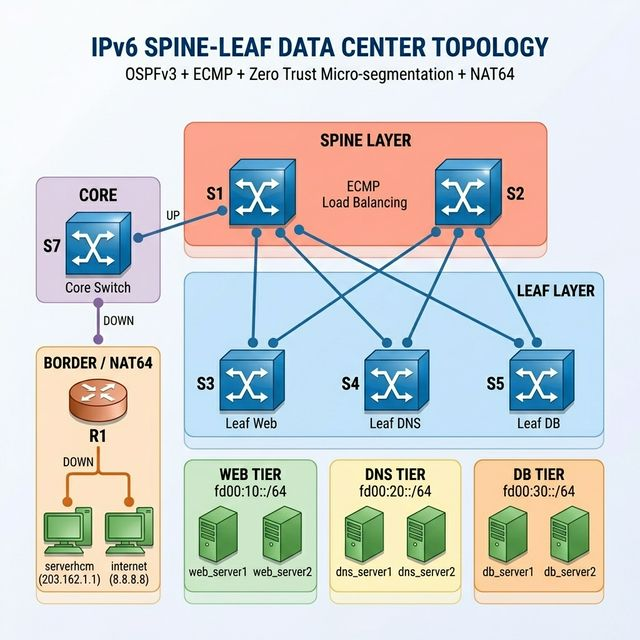
\includegraphics[width=\textwidth]{image/detailed_topology.png}
    \caption{Sơ đồ cấu trúc tổng thể IPv6 Spine-Leaf Data Center (với Public Host giả lập cho môi trường Internet).}
    \label{fig:detailed_topology}
\end{figure}

Toàn bộ hệ thống được mô phỏng trên nền tảng \textbf{Mininet} kết hợp bộ định tuyến mã nguồn mở \textbf{FRRouting (FRR)}, và được trang bị công cụ đo lường tự động để trích xuất số liệu khoa học.
